\documentclass{article}

\usepackage{graphicx}
\usepackage[colorlinks=true]{hyperref}
\usepackage[format=plain, labelfont=it, font=footnotesize, labelsep=period]{caption}
\usepackage[margin=1in]{geometry}
\usepackage{amsmath}
\usepackage{amssymb}
\usepackage{IEEEtrantools}

\renewcommand{\theequation}{\arabic{section}.\arabic{equation}}

\begin{document}

\begin{titlepage}
\vspace*{\stretch{1}}
\centering
\Huge Investigating the Mathematics behind Edge Detection
\vspace*{\stretch{1}}
\end{titlepage}

\tableofcontents
\newpage

\section{Introduction}
As a programmer and hobbyist graphic designer, I have worked with many vector and raster-based design programs ranging from Gravit Designer to Adobe Photoshop, and wondered about how certain features are implemented. Thus, I focused my attention to the mathematics governing algorithms used in 2D computer graphics, but my initial stages of research revealed many areas that could be potentially explored. However, I remember one day I tried to vectorize a photograph by tracing around it with the pen tool, which sparked my desire to explore how a computer would “trace” a photograph through edge detection.

\begin{figure}[!hbtp]
    \centering
    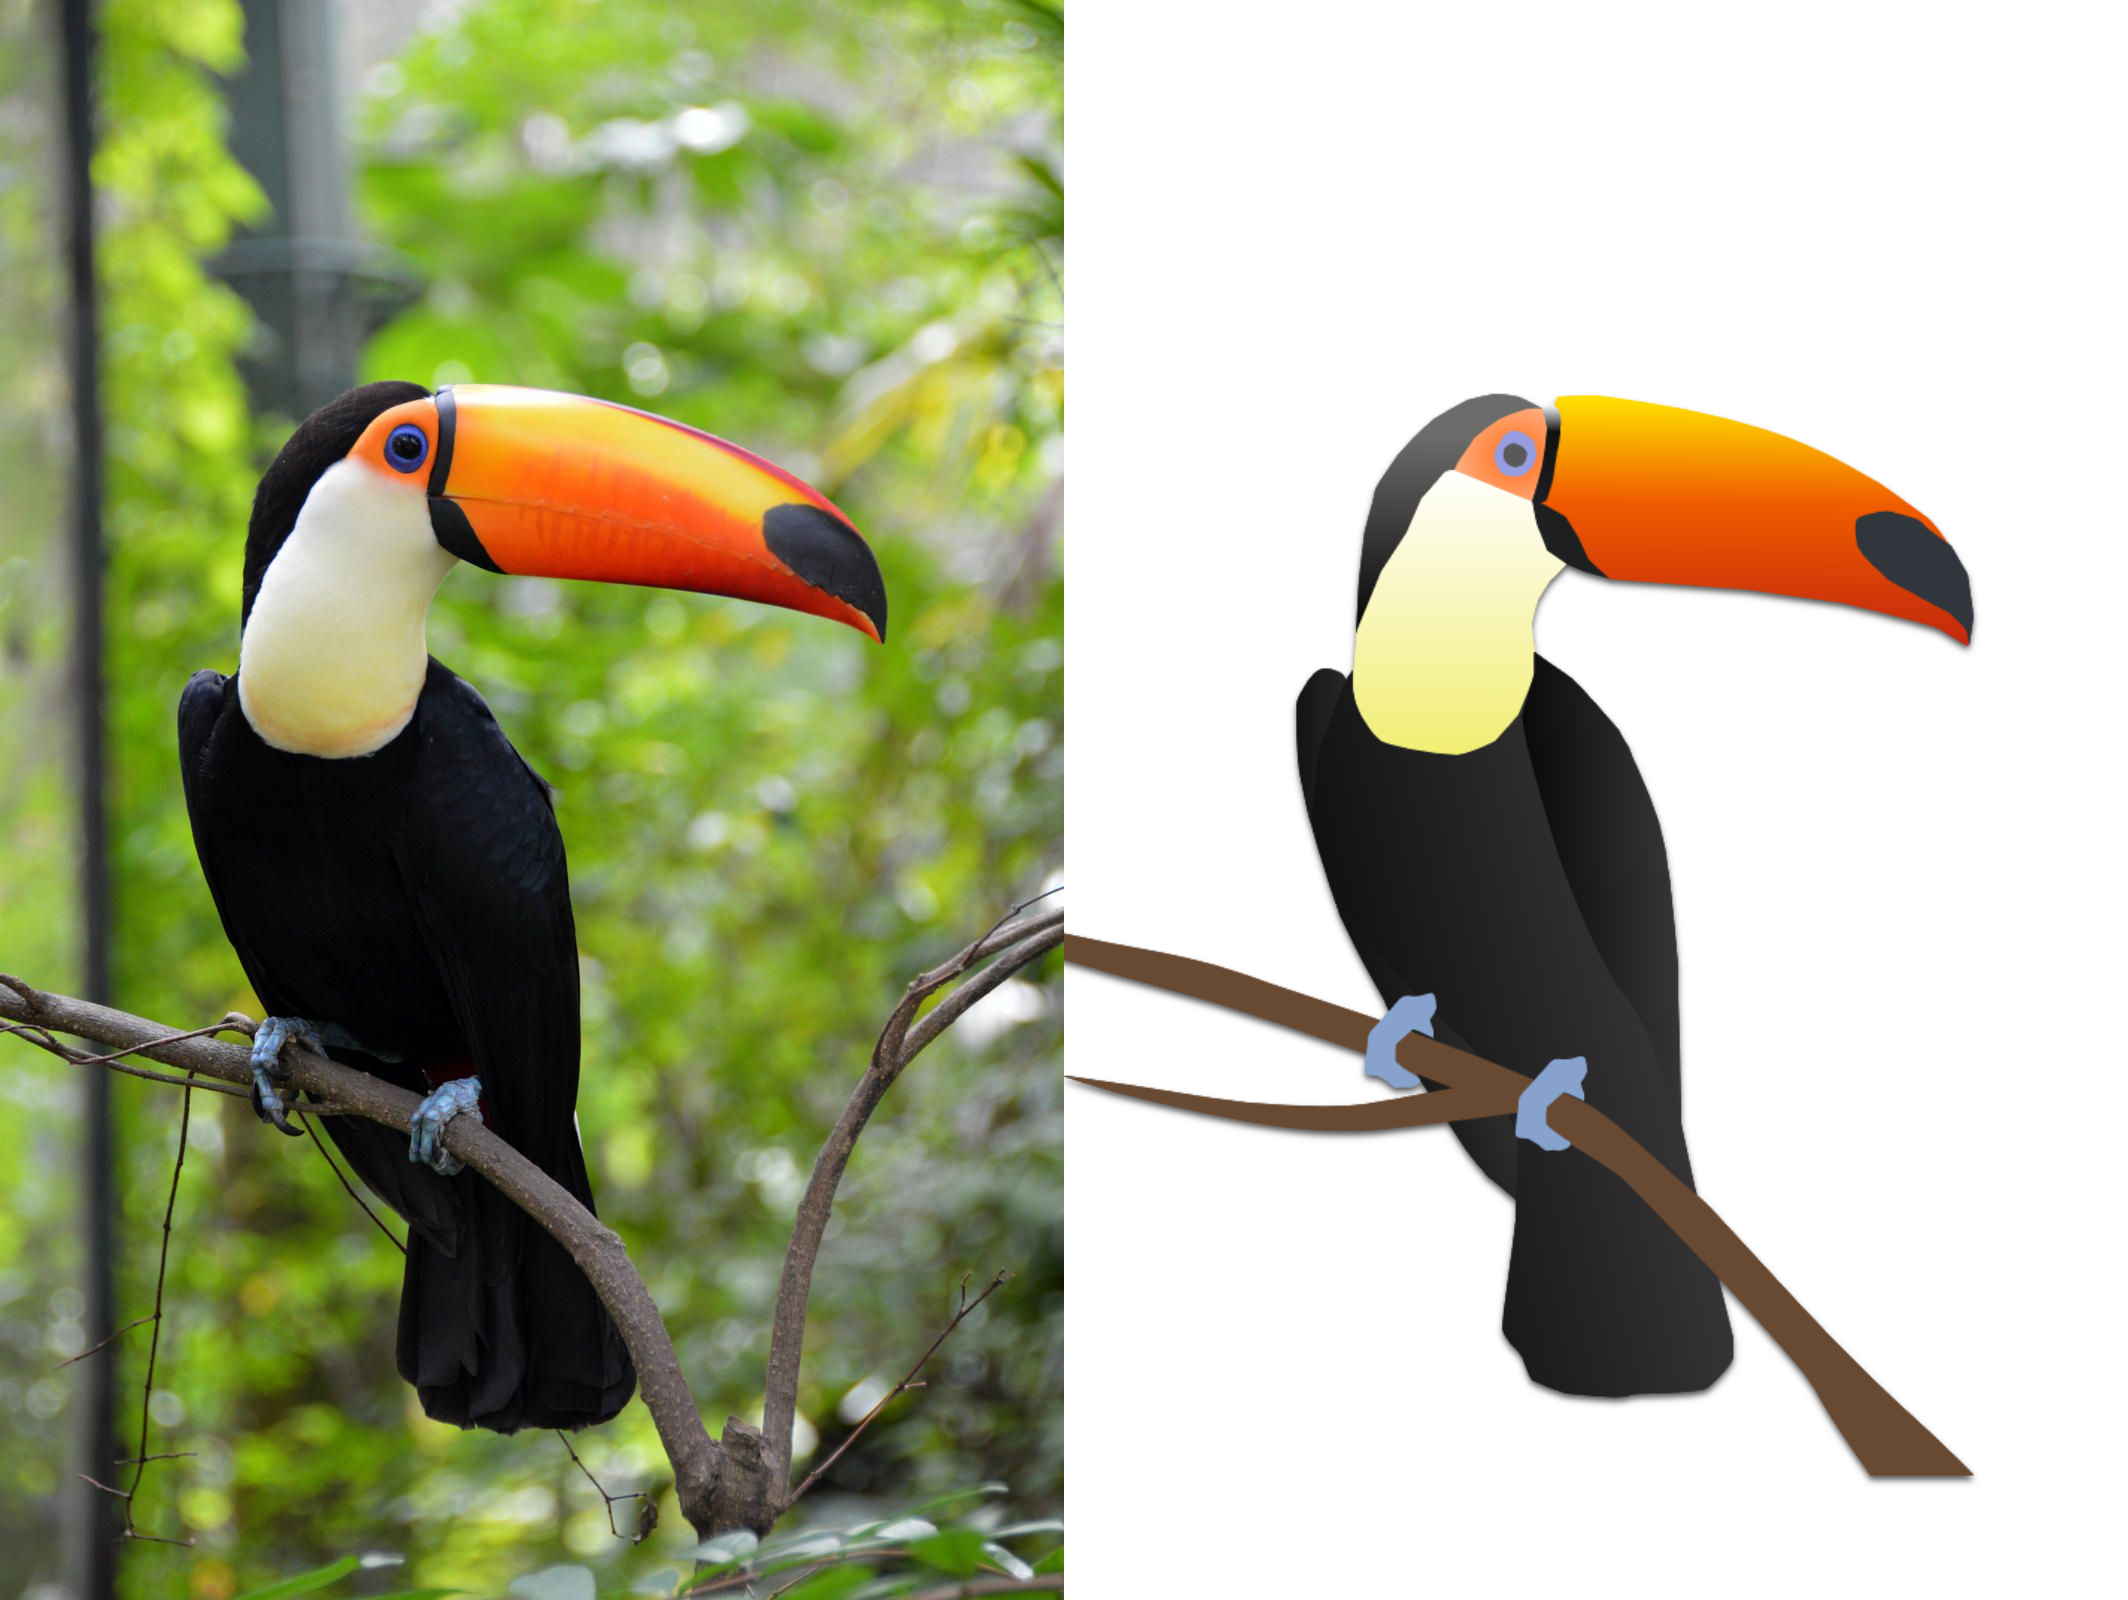
\includegraphics[width=\textwidth]{figures/figure01.png}
    \caption{\centering The exact image I tried to trace. Left image retrieved from \href{https://static.wikia.nocookie.net/maker-scratchpad-youtube/images/2/2a/Toco_Toucan.jpg/revision/latest?cb=20200318045659}{https:\slash\slash static.wikia.nocookie.net\slash maker-scratchpad-youtube\slash images\slash 2\slash 2a\slash Toco\_Toucan.jpg\slash revision\slash latest?cb=20200318045659}}
    \label{fig:figure 1}
\end{figure}

Otherwise specified, all images used for this maths exploration were taken or generated by me. Additionally, code used to generate some of these images can be found in the appendix. When coding, I tired to stay as far as possible from using external libraries that provided implementations for algorithms performed on images. This allowed me to thoroughly demonstrate my understanding of the mathematics involved in the concepts that will be discussed in my exploration.

\section{Images and Edges}
To a computer, an image represents a grid of pixels, each pixel containing a set of values that correspond to its colour. While it is easy for humans to detect edges by observing changes in color and pattern, a computer requires these changes in “colour and pattern” to be explicitly defined, that is, a sharp change or discontinuity in image intensity.

An image's colour does not influence a computer's ability to detect edges, so grayscale images suffice for edge detection. Therefore, a high image intensity represents a lighter pixel while a lower image intensity represents a darker pixel.

Edges can be categorized into 4 common types:

\begin{figure}[!hbtp]
    \centering
    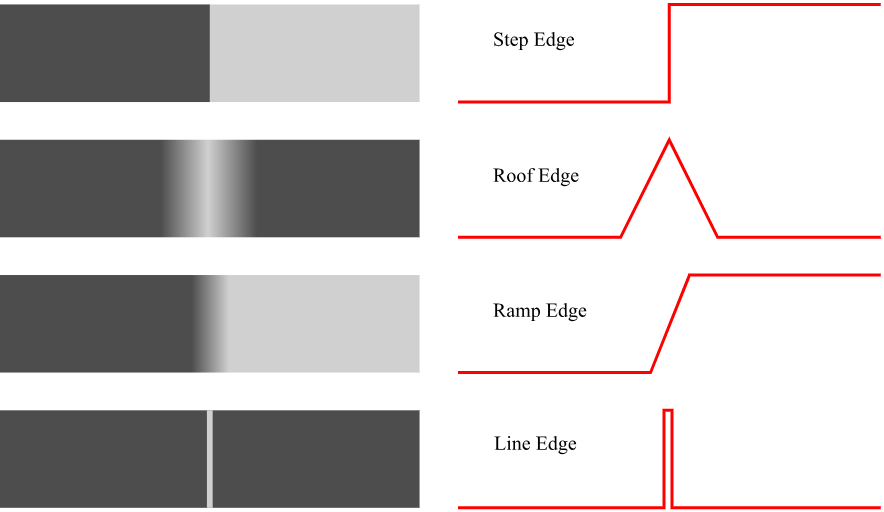
\includegraphics[width=\textwidth]{figures/figure02.png}
    \caption{\centering The 4 common types of edges. The left side gives a gives a visual representation of an edge while the right side shows the edge's intensity profile.}
    \label{fig:figure 2}
\end{figure}

Having established the definition of an edge, a mathematical way to detect them can be formed.

\section{The Discrete Derivative}
Recall that the definition of the derivative for a differentiable function is given by:
\begin{equation}
    \frac{df}{dx} = \lim_{h \to 0}{\frac{f(x+h) - f(x)}{h}}
\end{equation}
However, it is also useful to know that:
\begin{equation}
    \frac{df}{dx} = \lim_{h \to 0}{\frac{f(x+h) - f(x)}{h} = \lim_{h \to 0}{\frac{f(x) - f(x-h)}{h}} = \lim_{h \to 0}{\frac{f(x+h) - f(x-h)}{2h}}}
    \label{eqn:triple derivative}
\end{equation}

\newpage

Now consider the image intensity profile $I[x]$, a discrete function such that $\{I:I \in \mathbb{Z}, 0 \le I \le 255\}$ and $\{x:x \in \mathbb{Z}, 0 \ge 0\}$ where $I[x]$ denotes the image intensity at pixel $x$. Given the image below:

\begin{figure}[!hbtp]
    \centering
    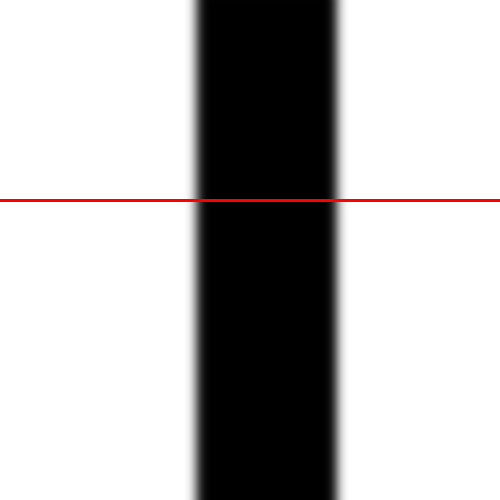
\includegraphics[width=0.5\textwidth]{figures/figure03.png}
    \caption{The intensity profile of this image is denoted by the red line}
    \label{fig:figure 3}
\end{figure}

The following graphs can be made:
\begin{figure}[!hbtp]
    \centering
    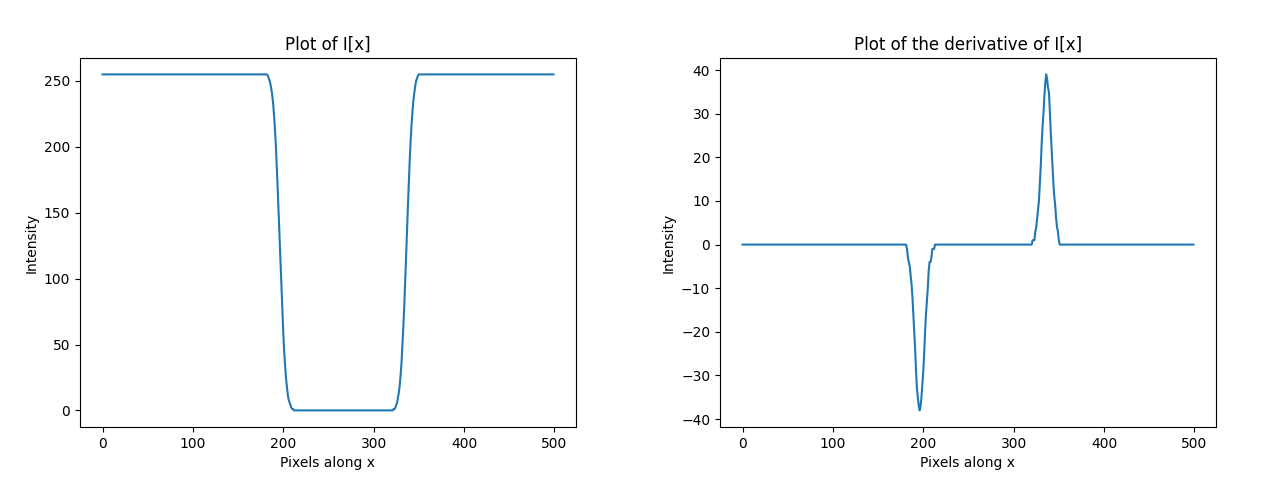
\includegraphics[width=\textwidth]{figures/figure04.png}
    \caption{Graphs for $I[x]$ and the derivative of $I[x]$}
    \label{fig:figure 4}
\end{figure}
Since an edge is defined as a sharp change in image intensity, taking the derivative of $I[x]$
effectively determines the location of edges. To take the derivative of the discrete function $I[x]$,
 the definition
\begin{equation*}
    \frac{dI}{dx} = \lim_{h \to 0}{\frac{f(x+h) - f(x)}{h} = \lim_{h \to 0}{\frac{f(x) - f(x-h)}{h}} = \lim_{h \to 0}{\frac{f(x+h) - f(x-h)}{2h}}}
\end{equation*}
can be rewritten as:
\begin{equation*}
    \frac{dI}{dx} = \lim_{h \to 1}{\frac{f[x+h] - f[x]}{h} = \lim_{h \to 1}{\frac{f[x] - f[x-h]}{h}} = \lim_{h \to 1}{\frac{f[x+h] - f[x-h]}{2h}}}
\end{equation*}
Although the values for these derivatives at a pixel $x$ may be different, they represent the same thing conceptually. The first 2 limits simply take the difference between adjacent pixel intensities while the 3rd takes the difference between the intensities of a pixel to the right of $x$ and a pixel to the left of $x$. However, the most practical way to represent $\frac{dI}{dx}$ is:
\begin{align}
    \frac{dI}{dx} &= \lim_{h \to 1}{\frac{I[x+h] - I[x-h]}{2h}} \nonumber \\
    &= \frac{I[x+1] - I[x-1]}{2} \nonumber \\
    &= I[x+1] - I[x-1]
    \label{eqn:di over dx initial def}
\end{align}
Since $\frac{dI}{dx}$ is taken while centered at $x$. Additionally, $I[x]$ can be automatically ignored for negative values of $x$, and the constant $\frac{1}{2}$ is disregarded because $\frac{dI}{dx}$ is sometimes multiplied by an arbitrary constant to brighten the lighter pixels anyway. Moreover, the range of $\frac{dI}{dx}$ is restricted such that $0 \le \frac{dI}{dx} \le 255$, meaning numbers out of bounds can either be ignored, rounded to their nearest endpoint, or normalized to fit within the bounds.

\section{Images and Partial Derivatives}
\setcounter{equation}{0}
An image accounts for the image intensity profiles $I[x]$ for all values of y within the image's dimensions, making it a 2D intensity map. This means that an image is a discrete function of both $x$ and $y$, meaning it can be represented as $I[x,y]$ where $\{I:I \in \mathbb{Z}, 0 \le I \le 255\}$, $\{x:x \in \mathbb{Z}, x \ge 0\}$, and $\{y:y \in Z, y \ge 0\}$. Additionally, $(x,y)=(0,0)$ denotes the top left pixel.

\begin{figure}[!hbtp]
    \centering
    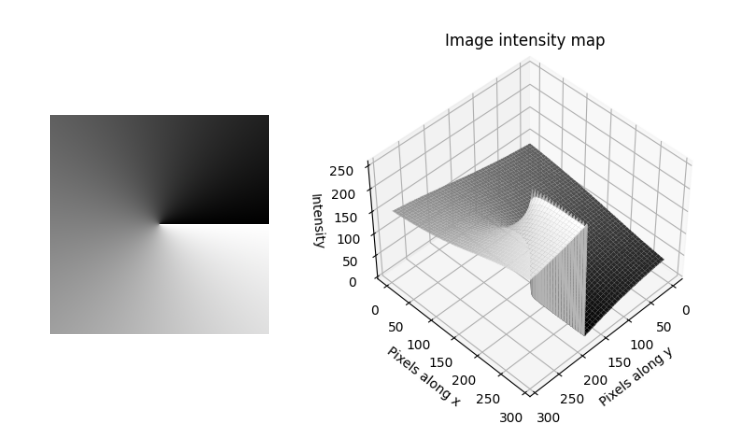
\includegraphics[width=\textwidth]{figures/figure05.png}
    \caption{Plotting the image intensity map for the image on the left}
    \label{fig:figure 5}
\end{figure}

It is useful to think in terms of derivatives again when detecting sharp changes in intensity. However, $I[x,y]$ may contain edges in any orientation, meaning the derivative of $I[x,y]$ in the $x$ and $y$ directions must both be considered. For a non-discrete function $f(x,y)$, taking the derivative with respect to one variable while holding the other constant is more formally known as the partial derivative.

The partial derivatives of $f(x,y)$ in the $x$-direction is given by:
\begin{equation}
    \frac{\partial f}{\partial x} = \lim_{h \to 0}{\frac{f(x+h, y) - f(x, y)}{h}}
\end{equation}
And in the $y$-direction:
\begin{equation}
    \frac{\partial f}{\partial y} = \lim_{h \to 0}{\frac{f(x, y+h) - f(x, y)}{h}}
\end{equation}
If applied to a discrete function like $I[x,y]$, $\frac{\partial f}{\partial x}$ can be represented as:
\begin{align}
    \frac{\partial I}{\partial x} &= \lim_{h \to 1}{\frac{I[x+h, y] - I[x, y]}{h}} \nonumber \\
    &= I[x+1, y] = I[x,y]
\end{align}
And $\frac{\partial f}{\partial y}$ as:
\begin{align}
    \frac{\partial I}{\partial y} &= \lim_{h \to 1}{\frac{I[x, y+h] - I[x, y]}{h}} \nonumber \\
    &= I[x, y+1] - I[x, y]
\end{align}
Once again, it is more practical to take $\frac{\partial f}{\partial x}$ and $\frac{\partial f}{\partial y}$ on $I[x, y]$ centered at the pixel $p(x, y)$. Following the logic in Equation \eqref{eqn:di over dx initial def} and extending it to 2D in the $x$-direction gives:
\begin{align}
    \frac{dI}{dx} &= \lim_{h \to 1}{\frac{I[x+h, y] - I[x-h, y]}{2h}} \nonumber \\
    &= \frac{I[x+1, y] - I[x-1, y]}{2} \nonumber \\
    &= I[x+1, y] - I[x-1, y]
    \label{eqn:di over dx initial def 2d}
\end{align}
Hence:
\begin{equation}
    \frac{dI}{dx} = I[x+1, y] - I[x-1, y]
\end{equation}

\newpage

Given the following image:

\begin{figure}[!hbtp]
    \centering
    
\includegraphics[width=0.5\linewidth]{figures/figure06.png}
    \caption{Ring shape consisting of only 3 shades of grey. The image size is 1000 pixels by 1000 pixels.}
    \label{fig:figur 6}
\end{figure}

Applying $\frac{\partial I}{\partial x}$ and $\frac{\partial I}{\partial y}$ gives:

\begin{figure}[!hbtp]
    \centering
    
\includegraphics[width=\linewidth]{figures/figure07.png}
    \caption{The image on the left reflects $\frac{\partial I}{\partial x}$ and on the right $\frac{\partial I}{\partial y}$}
    \label{fig:figure 7}
\end{figure}

Since the intensity difference between a black and white pixel can be $\pm255$, the values for $\frac{\partial I}{\partial x}$ and $\frac{\partial I}{\partial y}$ are both within the range $[-255,255]$. However, the intensity values in Figure \ref{fig:figure 7} were normalized to fit within the range $[0,255]$ by applying the following formula to the image intensity $I[p]$ at each pixel $p(x,y)$, where $m_0$ and $M_0$ represent the minimum and maximum of the original range, respectively:
\begin{equation}
    I_\text{norm} = 255 \left( \frac{I[p] - m_0}{M_0 - m_0} \right) \nonumber
\end{equation}
Visually, if $I[p]$ is closer to $m_0$, $I_\text{norm}$ is closer to 0 (hence darker) and if $I[p]$ is closer to $M_0$, then $I_\text{norm}$ is closer to 255 (hence lighter).

\section{The Gradient Vector and the Directional Derivative}
\setcounter{equation}{0}

Figure \ref{fig:figure 7} depicts edges being successfully detected in the $x$ and $y$ directions. If edges are to be detected in any direction, an important property of partial derivatives must be applied. Consider a point $p(x,y)$ on a function $f(x,y)=f(p)$ with partial derivatives $\frac{\partial f}{\partial x}$ and $\frac{\partial f}{\partial x}$. The gradient vector of the function, $\nabla f(p)$ is defined as a vector with $x$ and $y$ components $\frac{\partial f}{\partial x}$ and $\frac{\partial f}{\partial y}$:
\begin{equation}
    \nabla f(p) = \begin{pmatrix}
        \frac{\partial f}{\partial x} \\[1ex]
        \frac{\partial f}{\partial y}
    \end{pmatrix}
\end{equation}
For example, $\nabla f(p)$ for the function $f(p) = x^2 + y^2$ generates a vector field along the $xy$-plane governed by:
\begin{align}
    \nabla f(p) &= \begin{pmatrix}
        \frac{\partial}{\partial x} (x^2 + y^2) \\[1ex]
        \frac{\partial}{\partial y} (x^2 + y^2)
    \end{pmatrix} \nonumber \\
    &= \begin{pmatrix}
        2x + 0 \\
        0 + 2y
    \end{pmatrix} \nonumber \\
    &= \begin{pmatrix}
        2x \\
        2y
    \end{pmatrix}
\end{align}
The graph of $f(p)$ and $\nabla f(p)$ is simultaneously shown below:

\begin{figure}[!hbtp]
    \centering
    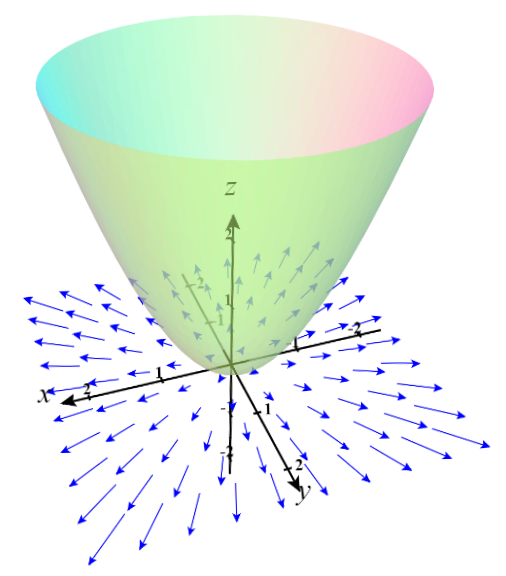
\includegraphics[width=0.5\linewidth]{figures/figure08.png}
    \caption{The paraboloid depicts $f(x,y)$ while the vector field depicts $\begin{pmatrix}2x\\2y\end{pmatrix}$. Image created with CalcPlot3D.}
    \label{figure 8}
\end{figure}

The visualization in Figure 8 provides an interesting observation, that is $\nabla f(p)$ for $f(x,y)=x^2+y^2$ always points in the direction of steepest ascent on the function. To prove that this is the case for any $f(x,y)$, the concept of the directional derivative is useful.

\end{document}

$\frac{\partial f}{\partial x}$
$\frac{\partial f}{\partial y}$

custom figures

proper indentation for paragraphs

double check equation formulas
